%%%%%%%%%%%%%%%%%%%%%%%%%%%%%%%%%%%%%%%%%%%%%%%%%%%%%%%%%%%%%%%%%%%%%%%%
%\cleardoubleevenemptypage
\chapter{Introduction}
\thispagestyle{noheadrule}
\markboth{}{}
\label{ch:intro}
%%%%%%%%%%%%%%%%%%%%%%%%%%%%%%%%%%%%%%%%%%%%%%%%%%%%%%%%%%%%%%%%%%%%%%%%
\pgfmathsetmacro\chapclr{\colourarray[1]} % set the number to the chapter number. Yes, by hand. Don't ask me why.
\hypersetup{
  citecolor  = \chapclr,
  linkcolor  = \chapclr,
  urlcolor   = \chapclr,
}

\epigraph{
  GROningen Mixture of Alchemy and Childrens' Stories
  }{
    \textit{from coolstuff.cpp}
}

\clearpage
%%%%%%%%%%%%%%%%%%%%%%%%%%%%%%%%%%%%%%%%%%%%%%%%%%%%%%%%%%%%%%%%%%%%%%%%%%
\section{Introduction}


I highly recommend to follow one sentence per line.

Contrary to popular belief, Lorem Ipsum is not simply random text.
It has roots in a piece of classical Latin literature from 45 BC, making it over 2000 years old.
Richard McClintock, a Latin professor at Hampden-Sydney College in Virginia, looked up one of the more obscure Latin words, consectetur, from a Lorem Ipsum passage, and going through the cites of the word in classical literature, discovered the undoubtable source.
Lorem Ipsum comes from sections 1.10.32 and 1.10.33 of "de Finibus Bonorum et Malorum" (The Extremes of Good and Evil) by Cicero, written in 45 BC.
This book is a treatise on the theory of ethics, very popular during the Renaissance. The first line of Lorem Ipsum, "Lorem ipsum dolor sit amet..", comes from a line in section 1.10.32.


\begin{center}
  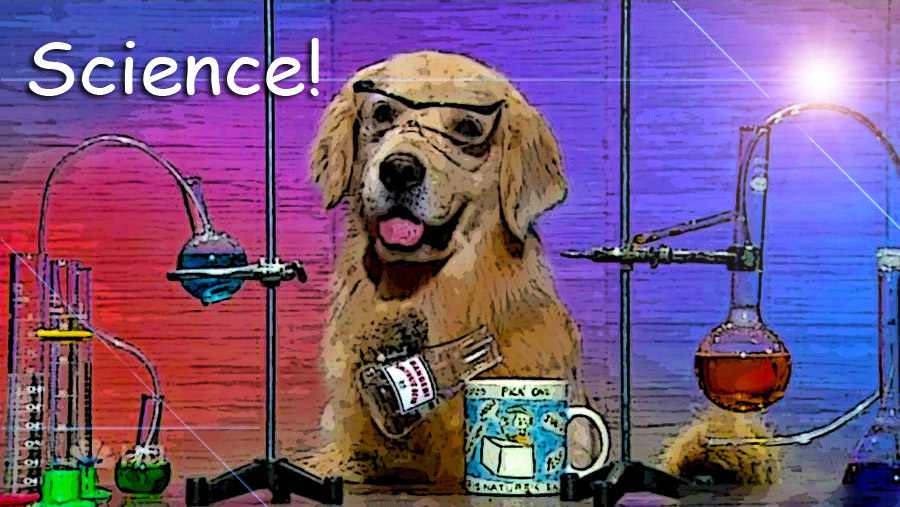
\includegraphics[width=1\linewidth]{sections/chapter1/Figures/dogs_do_science2.jpg}
  \captionof{figure}{\label{dogs_do_science}
  Give your caption here.
  }
\end{center}

\section{Some equations}
\begin{equation}
  \label{eqn:newtons}
  m_i \frac{d^2 \mathbf{r}_i}{dt^2} = \mathbf{F}_i(\mathbf{r}), \quad i=1,\ldots,N~.
\end{equation}
Here, $m_i$ and $\mathbf{r}_i$ are the mass and position of the $i$th atom, and $\mathbf{F}_i$ is the net force acting on that atom due to the presence of all other atoms.
The forces are the negative derivatives of a potential function $V(\mathbf{r}_1, \mathbf{r}_2, \ldots, \mathbf{r}_N)$:
\begin{equation}
  \mathbf{F}_i = -\frac{\partial V}{\partial \mathbf{r}_i}.
\end{equation}

\clearpage

\section{Outline of the thesis}
Write something here before starting the below.

\textbf{Chapter \ref{ch:chapter2}}  investigates the full-length tertiary structure and conformational dynamics of monomeric DNAJB6b.
Using homology modeling and microsecond-long all-atom molecular dynamics simulations, we show that DNAJB6b transitions between three conformational states: a closed state, an open state, and a less frequent extended state.
The closed and open states are the predominant conformations observed during the simulations.
Across all three states, the autoinhibitory state, i.e., the interdomain interaction between helix \croman{5} in the G/F domain and helices \croman{2} and \croman{3} of the J-domain remains intact, suggesting that the autoinhibitory mechanism persists in the absence of substrate, potentially preventing Hsp70 binding under non-stressed cellular conditions.

And do this for all chapters here.
